\Exercise[number={1}]
A dataset is described by a multivariate Gaussian probability density
function: \(x \sim \mathcal{N}(\mu, \Sigma)\) with \(\mu=[4,5]^T\)
and covariance matrix:
\begin{align*}
    \Sigma=
    \begin{bmatrix}
        5&&4\\4&&5
    \end{bmatrix}
\end{align*}
Draw the contour lines of the probability density function, determining
in particular its main directions.

\Answer[number={1}]
The covariance matrix is not diagonal, thus to draw the 2D contour lines of
the Gaussian distribution considered it is necessary to go through eigenvalue
decomposition, leading to \(\Sigma=USU^T\).
Firstly, it is necessary to compute the eigenvalues of the \(\Sigma\) matrix:
\begin{align*}
    \det{(\Sigma - \lambda I)} = 0
    \Rightarrow
    \begin{vmatrix}
        5-\lambda && 4 \\
        4 && 5-\lambda
    \end{vmatrix}
    =
    (5-\lambda)^2 - 16 = 0
    \Rightarrow
    \lambda_1 = 1, \lambda_2 = 9
\end{align*}
Therefore, the diagonal covariance matrix is
\(
    S
    =
    \begin{bmatrix}
        \lambda_1 && 0 \\
        0 && \lambda_2
    \end{bmatrix}
    =
    \begin{bmatrix}
        1 && 0 \\
        0 && 9
    \end{bmatrix}
\)
. \\
Now, the eigenvectors generating the matrix
\(
    U
    =
    \begin{bmatrix}
        u_{11} && u_{21} \\
        u_{12} && u_{22}
    \end{bmatrix}
\)
should be determined as follow:
\begin{align*}
    \Sigma u_1 = \lambda_1 u_1
    \Rightarrow
    \begin{bmatrix}
        5 && 4 \\
        4 && 5
    \end{bmatrix}
    \begin{bmatrix}
        u_{11} \\
        u_{12}
    \end{bmatrix}
    &=
    1
    \begin{bmatrix}
        u_{11} \\
        u_{12}
    \end{bmatrix}
    \Rightarrow
    u_{12}=-u_{11}
    \Rightarrow
    u_1=
    \begin{bmatrix}
        -\frac{1}{\sqrt{2}} && \frac{1}{\sqrt{2}}
    \end{bmatrix}
    \\
    \Sigma u_2 = \lambda_2 u_2
    \Rightarrow
    \begin{bmatrix}
        5 && 4 \\
        4 && 5
    \end{bmatrix}
    \begin{bmatrix}
        u_{21} \\
        u_{22}
    \end{bmatrix}
    &=
    9
    \begin{bmatrix}
        u_{21} \\
        u_{22}
    \end{bmatrix}
    \Rightarrow
    u_{22}=u_{21}
    \Rightarrow
    u_2=
    \begin{bmatrix}
        \frac{1}{\sqrt{2}} && \frac{1}{\sqrt{2}}
    \end{bmatrix}
\end{align*}
Leading to the eigenvectors matrix
\(
    U
    =
    \begin{bmatrix}
        -\frac{1}{\sqrt{2}} && \frac{1}{\sqrt{2}} \\
        \frac{1}{\sqrt{2}} && \frac{1}{\sqrt{2}}
    \end{bmatrix}
    =
    \frac{1}{\sqrt{2}}
    \begin{bmatrix}
        -1 && 1 \\
        1 && 1
    \end{bmatrix}
\)
.\\
At this point, let's write the probability density function of the multivariate
Gaussian distribution by assuming a random variable \(y\):
\[
    p(y;\mu,\Sigma)=(2\pi)^{-\frac{d}{2}}|\Sigma|^{-\frac{1}{2}}\exp{\biggl\{-\frac{1}{2}(y-\mu)^T\Sigma^{-1}(y-\mu)\biggr\}}
\]
The contour lines are \((y-\mu)^T\Sigma^{-1}(y-\mu) = constant\), then
the random variable can be changed by
\((y-\mu)=Ux \Rightarrow (Ux)^TUS^{-1}U^T(Ux)=x^T\cancel{U^TU}S^{-1}\cancel{U^TU}x=constant\)
as \(U\) is orthonormal, thus \(U^T = U^{-1} \Rightarrow U^TU=U^{-1}U=I\).\\
Finally, the expression
\(x^TS^{-1}x=
\begin{bmatrix}
    x_1 && x_2
\end{bmatrix}
\begin{bmatrix}
    1 && 0 \\ 0 && \frac{1}{9}
\end{bmatrix}
\begin{bmatrix}
    x_1 \\ x_2
\end{bmatrix}
=
\frac{x_1^2}{1}+\frac{x_2^2}{9}
=
constant
\)
is obtained.
The axes of the ellipse by assuming \(constant=1\) are calculated as
\(2\sqrt{\lambda_1}\) and \(2\sqrt{\lambda_2}\).
\begin{figure}[H]
    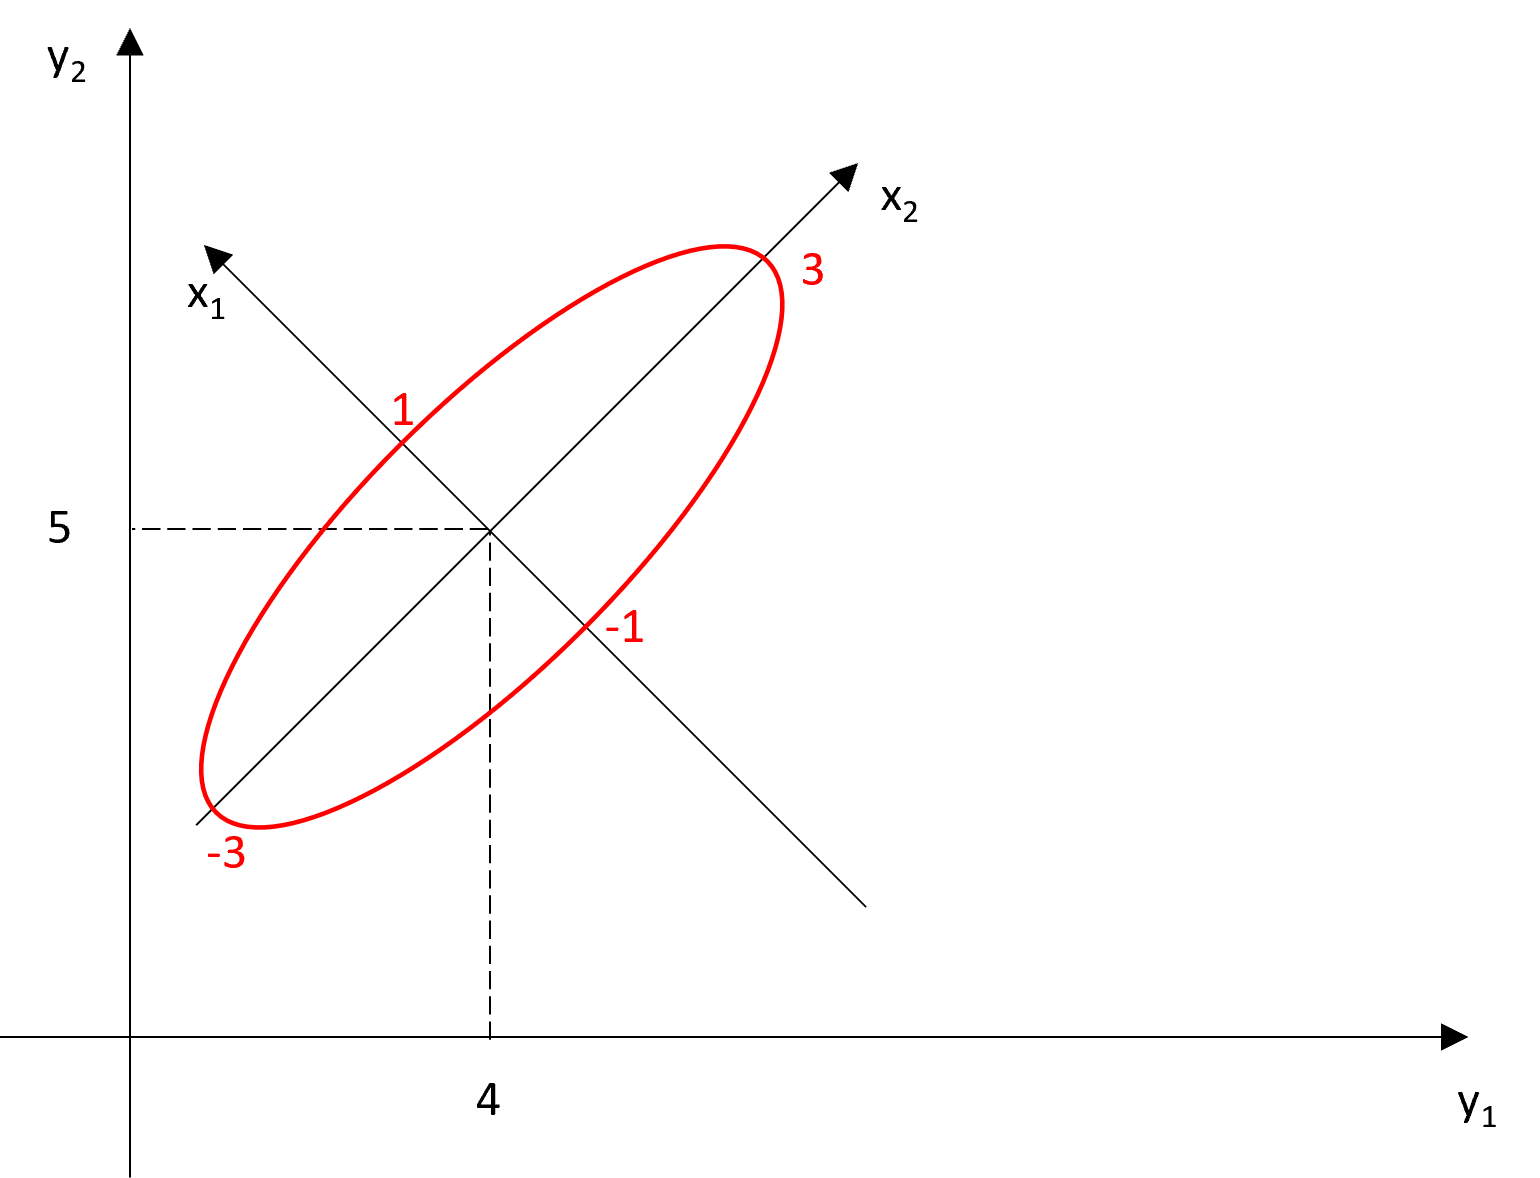
\includegraphics[scale=0.8]{B_1}
    \centering
\end{figure}